\documentclass[11pt]{article}
\usepackage{fullpage}
\usepackage{graphicx}

\title{Detecting Insults in Social Commentary}
\author{Andrew Conant and Fengjun (Jack) Yang}
\date{May 2016}

% Possible works cited:
% scikit learn
% unidecode

\begin{document}

\maketitle
\section{Introduction}
Internet comments: bastions of hatred and vitriol. While online anonymity has
provided a new outlet for aggression and hate speech, machine learning can be
used to fight it. The problem we sought to solve was the tagging of internet
comments that are aggressive towards other users. This means that insults to
third parties such as celebrities will be tagged as unoffensive, but "u are an
idiot" is clearly offensive. Additionally, broadly offensive rhetoric such as
racism and sexism regarding groups of individuals will not be tagged, as those
are beyond the scope of the project. 

To this end, classification algorithms are extremely effective and able to
learn to reasonably high degrees which comments are likely to offend online
participants.  In particular, we applied support vector machines (SVMs), random
forests, and naive Bayes to the problem, and in most cases found SVMs to be the
superior choice.  Additionally, we used several different vectorization
techniques involving both character and word n-grams (sequences of n characters
or words) before combining them into an ensemble classifier using a multi-layer
perceptron.

Advances in this area could be applied to social media, but the ethics and
effectiveness of such a prospect could be the subject of an entirely separate
paper.  However, this method shows promise (as a proof of concept), and some
more engineering could perhaps push towards a practical implementation.

\section{Method and Details}

\subsection{Data Set}
The data set came with three subsets, the training set, which contains 3974
samples, the test dataset, which contains 2648 samples, and the Imperium test
data set, which contains 2236 less typical samples.  All the data samples
contain two attribute fields and a single label field. The label can be either
0 or 1, where 0 denotes a non-insulting comment and 1 denotes an insulting one.
The first attribute is a (sometimes omitted) timestamp of the format
'YYYYMMDDhhmmss', while the second is the raw, unicode-escaped body of the
internet comment.

\subsection{Preprocessing}
Ultimately, the goal of this project's preprocessing step was to ensure that
semantically-identical words and phrases are grouped together by classifiers.
The first challenge was the removal of semantically meaningless text from the
comment bodies. For example, the data set is natively littered with ASCII
representations of unicode characters, such as \textbackslash xa0 (the
nonbreaking space). We solved this by first using Python's decode functionality
to convert it to unicode, and then using the module 'unidecode', capable of
converting unicode characters to their most similar ASCII brethren.  The next
step was to remove newlines and carriage returns (\textbackslash n and
\textbackslash r respectively), as well as backslash-escaped apostrophes. The
apostrophe removal helped to facilitate the next step: special cases.

Most obvious (and related to apostrophe removal) was converting contractions to
multi-word sequences, such as "can't" to "can not". Other changes like treating
"ur" as "your", "u" as "you", and "da" as "the" can help minimize
misclassification; consult classify.py to see the comprehensive list of
alterations that were made.  Because most of the substitutions were chosen by
eyeballing the parsed data, the only other particularly interesting
preprocessing step was shortening 3+ character sequences. Because no
grammatically-correct sequence of 3+ characters exists in English, shortening
them to 2 characters will never decrease semantic meaning.  For example, a
misspelling of "all" as "alll" could cause misclassification using the word
n-gram vectorization strategy.

See the results section for comparisons between the respective outputs for
doctored and raw text.

\subsection{Vectorizing the Texts}

To analyze the texts with machine learning algorithms, we first need to convert
them to a valid input format for such algorithms. The method we used here was
the conversion of a given piece of text into a vector using
bag-of-words(n-grams) representation. In this approach, we first collected a
set of words that appeared at least once in the training set, and then sorted
it into a specific order. Then, for a given text sample, we mapped it to a
vector such that each element is the number of occurrences of a corresponding
word in the sample. For example, if our training data set consists of two
samples, training data = \{'the first sentence', 'not the first first
sentence'\} and our vectorizer sorted the words in the order of their
appearance, i.e. ['the', 'first', 'sentence', 'not'], then after vectorization,
the vectorized data set would become vectorized data = \{[1,1,1,0],[1,2,1,1]\}.

In our implementation, the vectorization process is performed by
CountVectorizor from the sci-kit learn package. Note that the CountVectorizer
class ignores novel words in new input that did not appear in training set. So
for the example above, when we encounter the text 'a new sentence', it will be
vectorized as [0,0,0,1].

In our experiment, we used several different parameters settings. The
CountVectorizer class supports not only single-word vectorization, but also
n-grams(n-word phrases) vectorization. Additionally, it supports vectorization
with character-n-grams (strings of n characters) as the basic vectorization
elements. We discovered that when using bag-of-n-gram representation, $n=2$
(using bi-grams) provided visible improvements without slowing down the
training and classification process too much. For character n-grams, we found
such balance between accuracy and runtime at n in range (3,7). Results for
other parameters can be seen in the results section.

\subsection{Support Vector Machine}

Support Vector Machine(SVM) is a vector classifier that separates data into two
categories. SVMs known for their outstanding performance in high dimensions. In
our experiment, we employed the C-Support vector classifier SVC in sci-kit
learn library. One of the most important parameters in the SVC class is the
kernel type, which included linear, polynomial, radial basis function, sigmoid,
etc. We experimented on the four different kernels mentioned, and came to the
conclusion that linear kernel works best for our task. We used the sklearn
default for the rest of the parameters.

\subsection{Random Forest}

Random Forest is an ensemble learning technique that combines that result of
several random decision tree classifiers. Our implementation used the sklearn
RandomForestClassifier class. In our final implementation, all the parameters
were the default, except for the number of random decision trees included in
the random forest. We chose the number of decision trees to be $n = 9$ instead
of the $n = 10$ default, based on the result our experiment on random forest,
which is explained in more detail in the results section.

\subsection{Naive Bayes}

In our final implementation, we used a Multinomial Naive Bayes classifier with
its sklearn default parameters, which is included in the sklearn Naive Bayes
package. We arrived at this point after testing on all three of Bernoulli,
multinomial, and Gaussian naive Bayes classifiers. Multinomial Naive Bayes
classifier outperformed the other two algorithms significantly both in terms of
shorter training time and higher accuracy.

\subsection{Multi-Layer Perceptron as ensemble}

To combine the previous three classifiers (plus an additional character-gram
version of SVM), we used a perceptron. This is implemented by the MLPClassifier
class from the sklearn module. As the results section expands upon, the no
hidden layer model was the most effective. Other parameters were default, such
as the 'l-bfgs' weights optimization algorithm, an L2 penalty term of 0.00001,
and a user's guide-suggested randomization seed.

\section{Results}

\subsection{Preprocessing}

Because many different preprocessing steps were applied to the data, one can
observe the effects they had on classification accuracy by removing them. This
section seeks to quantify that change while demonstrating the power and
flexibility of sklearn.  Notice that while there is a strict increase in
accuracy post-preprocessing, sklearn is incredibly effective (in comparison) at
working with even the raw data.  Also, note the steep dropoff in accuracy on
the "secret" test set, released only after the fact by Imperium. This is
evidence of two equally likely possibilities: either the training set is not
representative of the Imperium set, or the test set is too similar to the
training set. In the second case, overfitting caused abnormally good
performance on the test set and poor performance on the Imperium set, while in
the first case, our algorithm learned a good model that could not be applied to
partially irrelevant data. To clarify, SVM data is from the word-gram model.

\begin{table}[h]
    \centering
    \begin{tabular}{|c| c c c c c c|} 
    \hline
     &Test RF &Test GNB &Test SVM &Imp. RF &Imp. GNB &Imp. SVM \\ [0.5ex] 
    \hline
    With prep. & 81.0\% & 82.3\% & 83.9\% & 64.8\% & 66.0\% & 73.5\% \\ 
    \hline
    Without prep. & 80.0\% & 81.8\% & 83.9\% & 61.4\% & 65.1\% & 71.0\% \\ 
    \hline
    \end{tabular}
    \caption{Comparison of Accuracy of Algorithms with and without Preprocessing}
\end{table}
              
\subsection{Vectorizing}

To examine the effect of different vectorization techniques on the accuracy of
our final result, we ran several tests using different vectorization parameters
with different n-gram ranges, and we tested using both n-grams and character
n-grams as the basic element of vectorization. The classifiers used were Random
Forest(RF) with $n = 10$ random decision trees, Gaussian Naive Bayes(GNB) with
default parameters, and SVM with a linear kernel. The classifiers were trained
on the training data set and tested on the test data set.

\begin{table}[h]
    \centering
    \begin{tabular}{|c| c c c|} 
    \hline
     & RF & GNB & SVM \\ [0.5ex] 
    \hline
    1-gram(single word) & 80.3\% &68.6\% & 82.5\%\\ 
    \hline
    1,2-gram & 79.5\% & 76.3\% & 83.7\% \\
    \hline
    1,2,3-gram&79.3\%&76.3\%&84.1\% \\
    \hline
    1,2,3,4-gram&79.5\%&76.1\%&84.1\% \\
    \hline\hline
    (1,4) chars&80.5\%&70.5\%&81.7\% \\ 
    \hline
    (4,7) chars&82.1\%&75.7\%&83.3\% \\
    \hline
    (1,7) chars&80.4\%&70.5\%&83.6\% \\ 
    \hline
    \end{tabular}
    \caption{Comparison of Accuracy of Different Vectorization Parameters (slightly
              weaker preprocessing than final )}
\end{table}

As can be seen in the table, as the range of n-grams included in the
vectorization expanded, the accuracy in general also increased. This is
reasonable as increase in the dimensions provided new information that were not
represented with low dimensions. However, at the same time, the data also gave
us a peak at the negative effect of the curse of dimensionality. As we can see,
when n-gram range increased from (1,7) for character vectorization, the
accuracy became actually lower than that of n-gram range (4,7) except for SVM.
We suspect that this is because having too many dimensions clouded the
judgement of RF and GNB classifiers. At the same time, we also see that SVM
handles high-dimensional data better than the other two, as its accuracy kept
increasing as more dimensions were added.

\subsection{Support Vector Machine}

As mentioned in previous sections, sklearn support vector machine has different
kernels at our disposal. In this experiment, we tested the performance of
different kernels on our task. The results were run on texts vectorized as
bi-gram words, and trained on the training data set.

\begin{table}[h]
    \centering
     \begin{tabular}{|c| c c c c|} 
     \hline
      & Linear & Poly & RBF & Sigmoid \\ [0.5ex] 
     \hline
     Test data set & 83.7\% &73.8\% & 73.8\% & 73.8\%\\ 
     \hline
     Imperium data set & 72.0\% & 51.8\% & 51.8\%& 51.8\% \\
     \hline
    \end{tabular}
    \caption{Comparison of Results of SVMs with Different Kernels (slightly weaker
                preprocessing than final)}
\end{table}

As we can see, the results of linear kernel outperforms other kernals by a
large amount. We suspect that in our example, a linear kernel demonstrated such
performance because it mitigated overfitting.

\subsection{Random Forest}

As ensemble learning, the Random Forest classifier combines the results of
several individual random decision trees. In our experiment, we varied the
number of decision trees included in the random forest classifier and collected
data for the accuracy of random forest classifier with different number of
decision trees.

All of the random forest classifiers in this experiment are trained on the
training data set, with a bi-gram word vectorizer. Considering the
probabilistic nature of the random forest algorithm, the validation tests were
run 50 times before the average accuracy was taken. Figure.1 and Figure.2 shows
the accuracy change related the change of number of trees. The results in
Figure.1 were collected from testing on the test data set, while the results in
Figure.2 were from tests on the Imperium data set.

\begin{figure}[h]
    \centering
    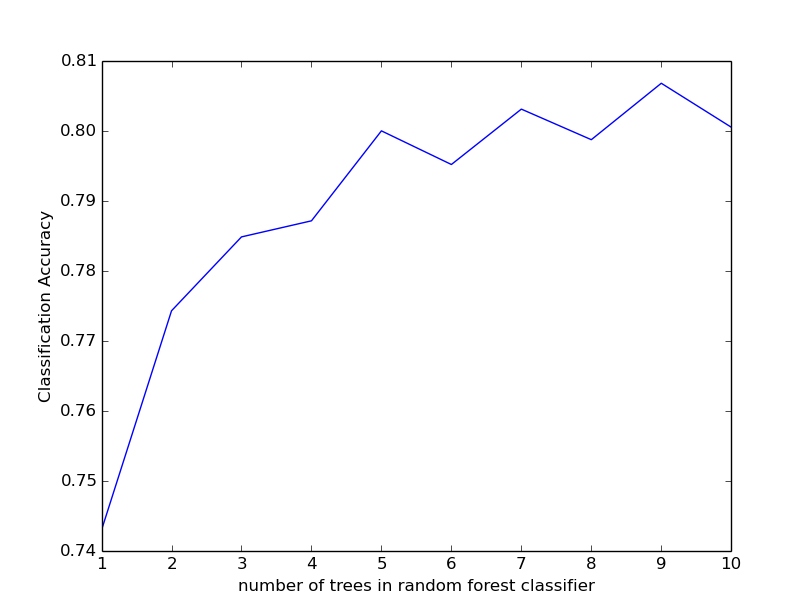
\includegraphics[scale=0.5]{RF_50run_test.png}
    \caption{Random Forest Accuracy with Varying Number of Random Decision Trees on Test Data Set}
    \label{fig:my_label}
\end{figure}

\begin{figure}[h!]
    \centering
    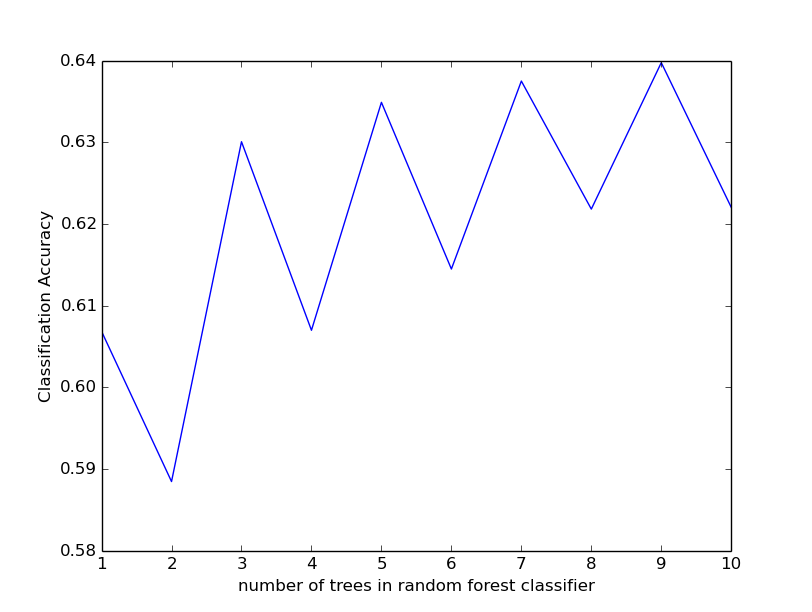
\includegraphics[scale=0.5]{RF_50run_imperium.png}
    \caption{Random Forest Accuracy with Varying Number of Random Decision Trees on Imperium Data Set}
    \label{fig:my_label}
\end{figure}

As we can see, the overall accuracy improves as the number of the classifiers
in the ensemble increases. However, in our case, the slope of accuracy
improvement flattens significantly when the number of trees exceeds n = 5. In
general, the ensemble classifier outperforms its individual components by a
significant amount. However, the marginal benefit of having one more random
decision trees decreases as the number of decision trees in the random forest
increases.

One interesting result from our experiment is that having odd number of trees
performs better than having even number of decision trees. We do not yet have
an explanation on why this result holds true. We suspect it might be related to
the fact that tie-breaking is easier when an odd-number of decision trees are
included.

\subsection{Multi-Layer Perceptron as Ensemble}

After training the individual classifiers, we trained a multi-layer perceptron
using the outputs of the four classifiers as inputs. In most cases, the
perceptron was only able to consistently classify with greater accuracy than
its best input when it had no hidden layers. Table 3 depicts the accuracy of
the perceptron with varying numbers of hidden layers of varying complexity. For
example, a tuple (5, 2) denotes two hidden layers, with the first containing
five neurons and the second containing two.  Additionally, the 'best
individual' column displays the best accuracy displayed by an individual
classification algorithm for that data set. In all cases it was from SVM with
word-grams.

\begin{table}[h]
    \centering
     \begin{tabular}{|c| c c c c c|} 
     \hline
      & () & (2,) & (5,) & (5,2) & Best individual\\ [0.5ex] 
     \hline
      Test data set & 84.6\% & 73.8\% & 84.1\% & 83.0\% & 83.9\% \\ 
     \hline
      Imperium data set & 73.6\% & 51.8\% & 72.6\% & 74.1\% & 73.5\% \\ 
     \hline
    \end{tabular}
    \caption{Comparison of Results for Multi-Layer Perceptron}
\end{table}

Because picking hidden layer setups for neural nets is such an inexact science,
we can only guess at the significance of these findings. This problem is so
prone to overfitting that it is possible that there is no universally correct
setup for hidden layers. By what may be a fluke, some of the hidden layer
configurations outperformed their individual parts, while others crashed and
burned.

\section{Conclusions}

We explored four different machine learning techniques and different
vectorization paradigms for the task of insult detection in text. We found that
linear kernel SVM has outstanding performance, thanks to its ability to
function in high dimensions. We also noticed that we can increase the accuracy
of the random forest classifier by increasing the number of composing random
decision trees. For our task, multinomial naive Bayes classifier performs
better than Gaussian and Bernoulli naive Bayes classifiers. Finally, we
integrated the results of these three classifiers with a multilayer perceptron,
and managed to produce a higher accuracy than any of the three classifiers
individually. Our final ensemble classifier achieve 84.6\% and 73.6\% accuracy
on the test data set and the Imperium data set respectively. Our work also left
interesting questions for future works to focus on. These questions include,
but are not limited to, the peculiar property of random forest performing
better with odd number of components, and the reason linear kernel achieves
better result than its counterparts. Analyzing these questions may provide
insight to further improve the accuracy for insult detection.

\end{document}
